\section{IAFoosball}
IAFoosball is the name of the project and startup we developed in the previous semester. It is meant to make foosball more interactive, to show and share statistics, and make it more sociable by using new technologies. The planned services include global and private rankings, table finder, friends, automatic tournaments and more. Because it is part of an university project, we used the latest and greatest technology. The front end is written in Flutter and pReact, the back end is separated in containerized microservices written in Go and all communication is done through gRPC, which uses protobuffs and HTTP/2. \Cref{fig:architectureCurr} shows this architecture.

\begin{figure}[h!]
    \centering
    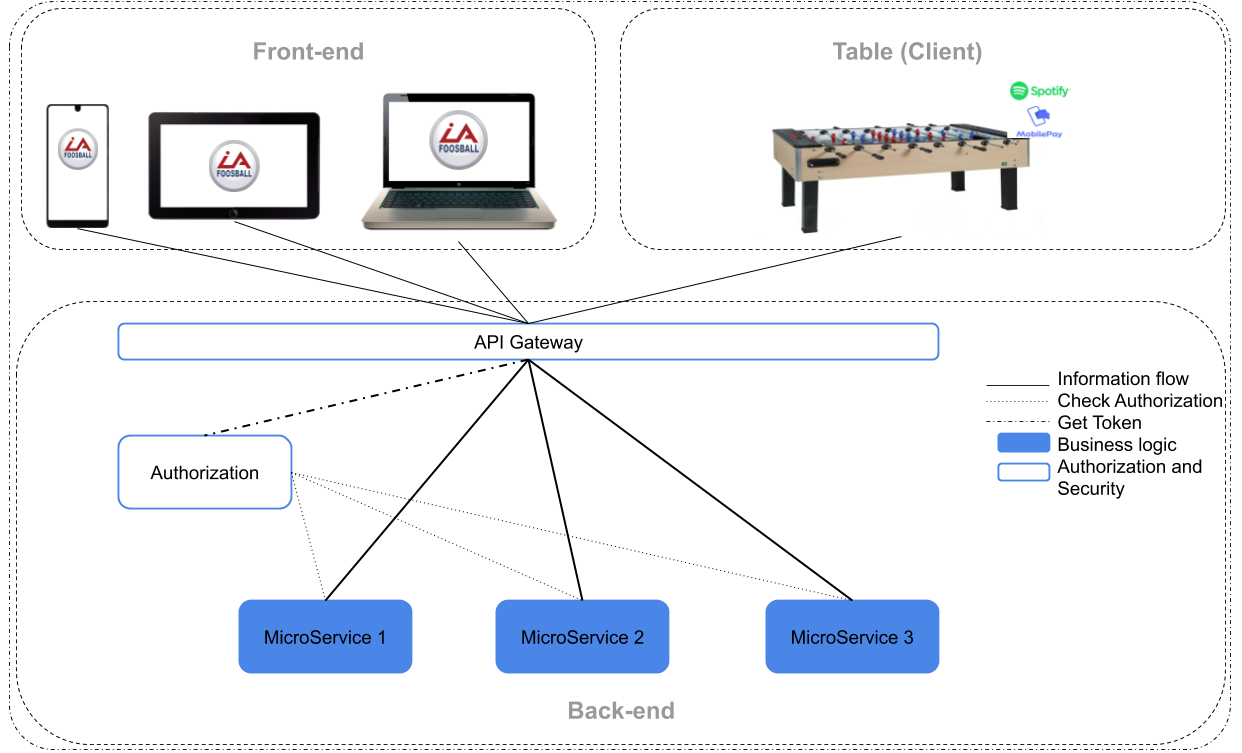
\includegraphics[scale=0.2]{figures/architecture-old.png}% picture filename
    \caption{The current IAFoosball architecture}\label{fig:architectureCurr}
\end{figure}

The foosball table in seen in \cref{fig:overview_table} 

\begin{figure}[h!]
    \centering
    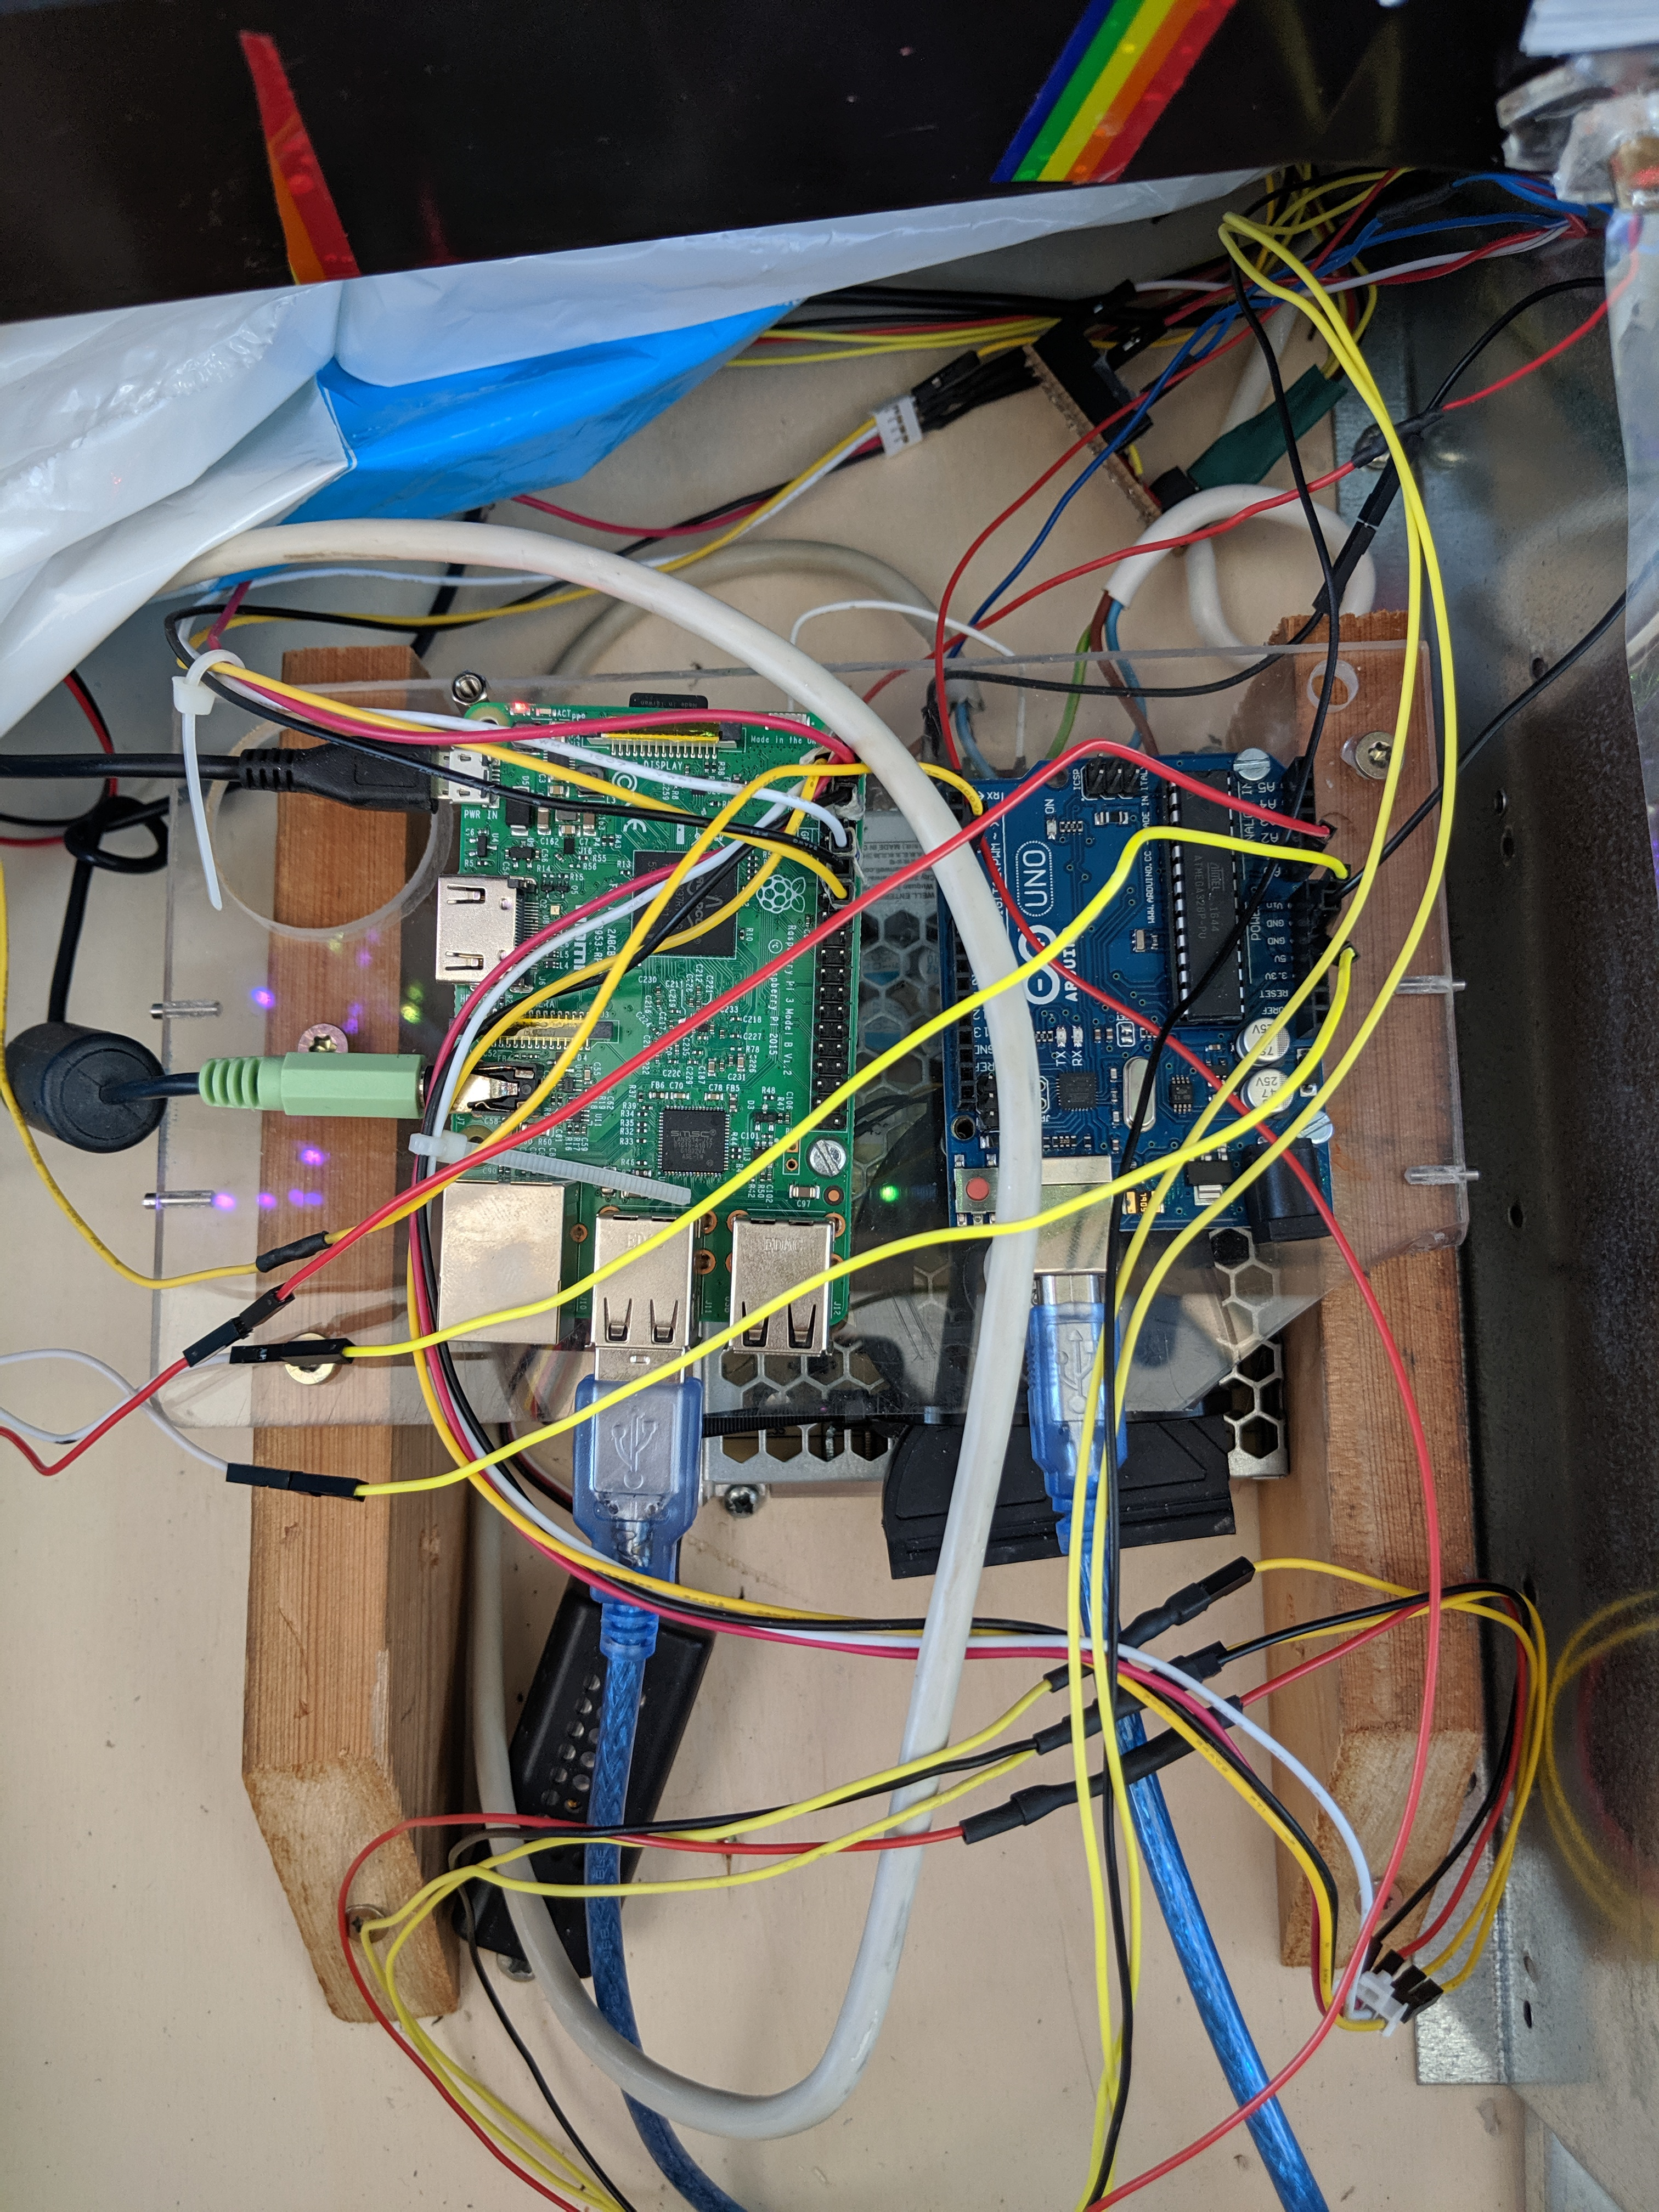
\includegraphics[scale=0.09]{figures/overview_table.jpg}}% picture filename
    \caption{The current IAFoosball table hardware}\label{fig:overview_table}
\end{figure}
In \cref{fig:overview_table} the development version can be seen, and has all features. It includes, speakers with Spotify integration, LED lights, automatic ball release and a tablet. However, the software and hardware used on the table does not life up to the software standards at IAFoosball. The software needs to be updated locally without a CI/CD (continous integration and continous delivery) pipeline and is attached physically to the IoT gateway, the raspberry pi. This makes it very hard to scale and not mainstream suitable. To make IAFoosball more compelling for people and business which just want goal counting, and possibly ball speed measurments, we wanted to cut down on features and instead concentrate on quality.\\


\subsection{Goal Design}
The goal design is the primary part of this report and the most lacking part in the former project. 
In \cref{fig:goalOld} the old electronic wiring is shown.

\begin{figure}[h!]
    \centering
    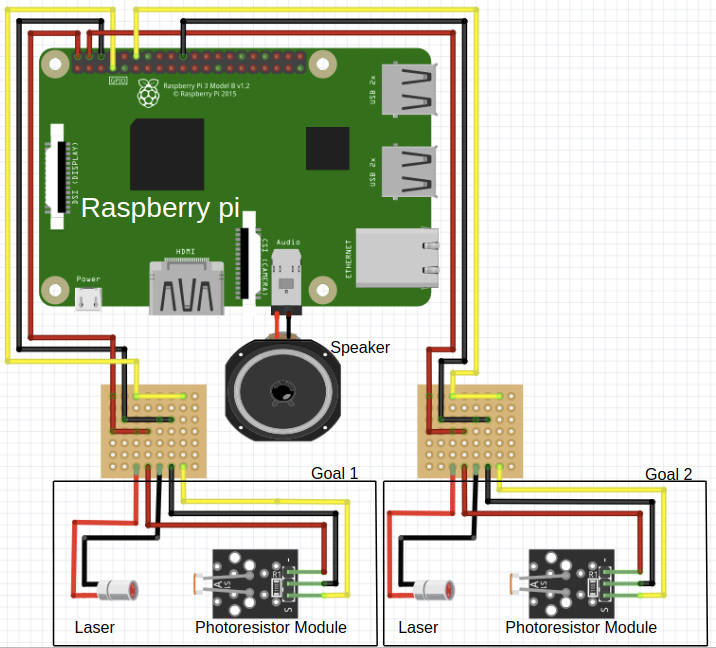
\includegraphics[scale=0.3]{figures/goal-old.png}
    \caption{The old IAFoosball goal}\label{fig:goalOld}
\end{figure}

The sensors were directly connected to Raspberry Pi, and a simple javascript application registered the goals and sent them to a remote server. This required a power outlet and a Raspberry Pi on each table. It also required cables from each goal to the Raspberry Pi. This approach did not scale well and in a multi-table setup also wasted money as each table needed its own Raspberry Pi. We re-thought the design, making it more versatile, easier to integrate and manage and also cheaper for multiple tables.

\begin{figure}[h!]
    \centering
    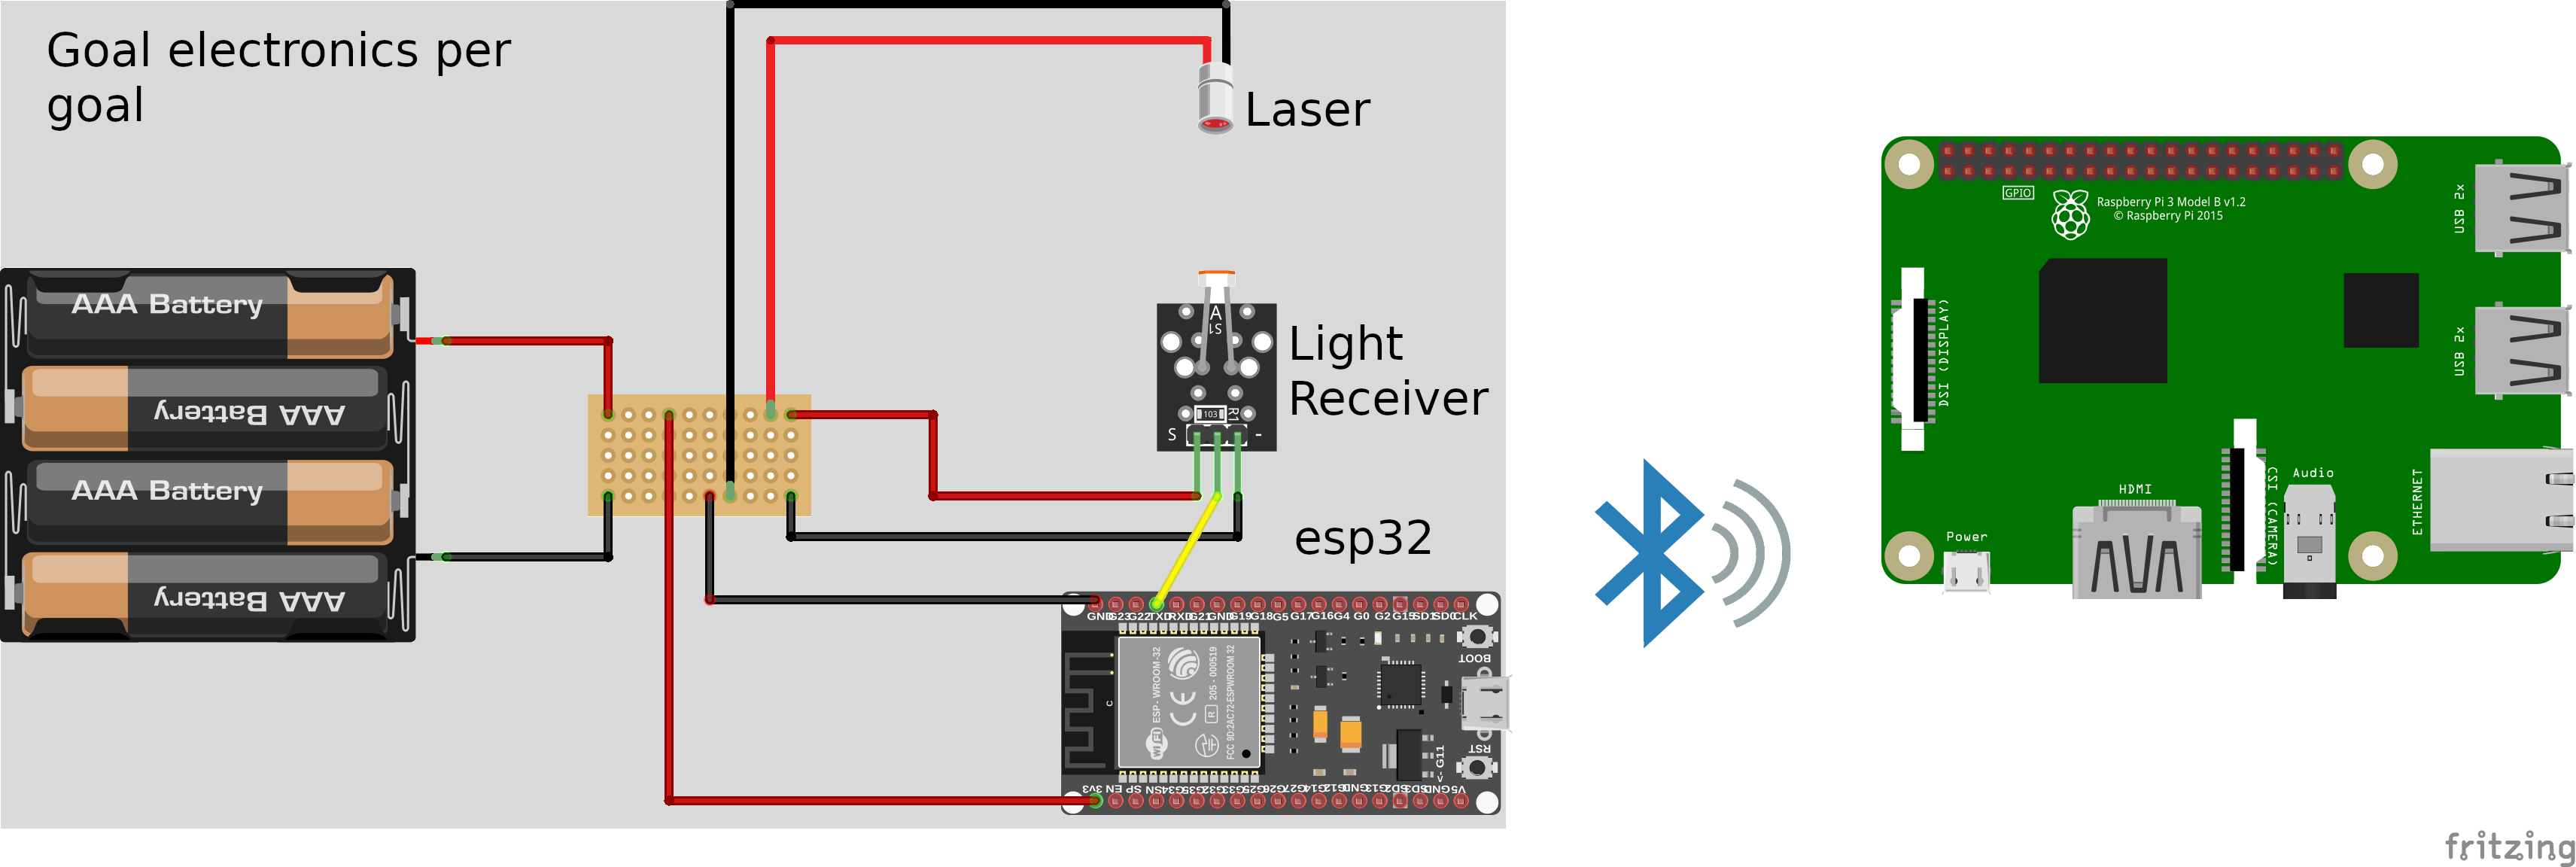
\includegraphics[scale=0.4]{figures/goal-new.png}% picture filename
    \caption{The new IAFoosball goal}\label{fig:goalNew}
\end{figure}

\Cref{fig:goalNew} show one option of this new setup. Marked in grey are the components used for each goal, a battery (we use a lithium-ion battery), one laser, one light sensor and one esp32. In this setup, the laser and sensors, and the esp32 are powered seperately and the esp32 has no control of the laser and sensor. We will discuss an alternative approach in the chapter Gaol Design. To measure goal speed we would need to have to lasers and two sensors. The esp32 is the component doing the computation and sending data to a Raspberry Pi via bluetooth low energy (BLE). It is powered by a battery pack and only active when the need arises.\\

